\documentclass[11pt]{article}
\usepackage[round,comma,authoryear]{natbib}
\usepackage{fullpage}
\usepackage{authblk}
\usepackage{graphicx}
\usepackage{booktabs}
\usepackage{amsmath}
\usepackage[labelformat=simple]{subcaption}

% Use upper case letters for subfigure captions.
\renewcommand{\thesubfigure}{\Alph{subfigure}}

\usepackage[newfloat]{minted}
\usepackage{tcolorbox}
\usepackage{etoolbox}
\BeforeBeginEnvironment{minted}{\begin{tcolorbox}}
\AfterEndEnvironment{minted}{\end{tcolorbox}}
\usepackage{url}
\usepackage{fancyvrb}
\usepackage{caption}
\newenvironment{code}{\captionsetup{type=listing}\centering}{}
\SetupFloatingEnvironment{listing}{name=Demographic Model}
% can either input code directly in a minted environment
% or input from a source file using \inputminted

% Import this last to avoid mysterious errors.
\usepackage[implicit=false]{hyperref}

% local definitions
\newcommand{\ms}[0]{\texttt{ms}}
\newcommand{\msprime}[0]{\texttt{msprime}}
\newcommand{\stdpopsim}[0]{\texttt{stdpopsim}}
\newcommand{\demes}[0]{\texttt{demes}}
\newcommand{\demesdraw}[0]{\texttt{demesdraw}}
\newcommand{\Demes}[0]{\texttt{Demes}}
\newcommand{\moments}[0]{\texttt{moments}}
\newcommand{\dadi}[0]{\texttt{dadi}}
\newcommand{\fwdpy}[0]{\texttt{fwdpy11}}
\newcommand{\slim}[0]{\texttt{SLiM}}
\newcommand{\gadma}[0]{\texttt{GADMA}}
\newcommand{\tskit}[0]{\texttt{tskit}}
\newcommand{\MSMC}[0]{\texttt{MSMC}}
\newcommand{\demesslim}[0]{\texttt{demes-slim}}

\newcommand{\aprcomment}[1]{{\textcolor{blue}{APR: #1}}}
\newcommand{\jkcomment}[1]{{\textcolor{red}{JK: #1}}}
\newcommand{\ggcomment}[1]{{\textcolor{yellow!60!red}{GG: #1}}}
\newcommand{\krtcomment}[1]{{\textcolor{purple}{KRT: #1}}}
\newcommand{\mhcomment}[1]{{\textcolor{cyan}{MH: #1}}}

\usepackage{catchfile}
\begin{filecontents*}{software-table.tex}
\end{filecontents*}

\begin{document}

\title{Demes: a standard format for demographic models}
% First authors
\author[1,$\star$]{Graham Gower}
\author[2,$\star$]{Aaron P. Ragsdale}

% Authors: please add your name and affiliation here, in alphabetical order.
% Second Authors
\author[3]{Ryan N. Gutenkunst}
\author[4]{Matthew Hartfield}
\author[5]{Ekaterina Noskova}
\author[8]{Stephan Schiffels}
\author[3]{Travis J. Struck}
%Senior Authors
\author[6,$\dagger$,$\aleph$]{Jerome Kelleher}
\author[7,$\dagger$]{Kevin R. Thornton}

\affil[1]{Section for Molecular Ecology and Evolution, Globe Institute, University of Copenhagen}
\affil[2]{Department of Integrative Biology, University of Wisconsin--Madison}
\affil[3]{Department of Molecular and Cellular Biology, University of Arizona}
\affil[4]{Institute of Ecology and Evolution, The University of Edinburgh}
\affil[5]{Computer Technologies Laboratory, ITMO University}
\affil[6]{Big Data Institute, Li Ka Shing Centre for Health Information and
    Discovery, University of Oxford}
\affil[7]{Ecology and Evolutionary Biology, University of California, Irvine}
\affil[8]{Max Planck Institute for Evolutionary Anthropology, Leipzig, Germany}

\affil[$\star$]{Denotes shared first authorship, listed alphabetically}
\affil[$\dagger$]{Denotes shared senior authorship, listed alphabetically}
\affil[$\aleph$]{Denotes corresponding author}


\maketitle

\begin{abstract}
Understanding the demographic history of populations is a
key goal in population genetics, and with improving methods
and data, ever more complex models are being proposed and tested.
Demographic models of current interest
typically consist of a set of discrete populations,
their sizes and growth rates, and continuous and pulse migrations
between those populations over a number of epochs, which can require
dozens of parameters to fully describe. There is currently
no standard format to define such models, significantly
hampering  progress in the field. In particular, the important
task of translating the model descriptions in published
work into input suitable for population genetic simulators is labor intensive
and error prone.
We propose the Demes data model and file format,
built on widely used technologies,
to alleviate these issues. Demes provides a well-defined and unambiguous
model of populations and their properties that is straightforward to
implement in software, and a text file format that is designed for
simplicity and clarity.
We provide thoroughly tested implementations of Demes parsers
in multiple languages including Python and C,
and showcase initial support in several simulators and inference
methods.
An introduction to the file format and a detailed specification are available at:\\
\url{https://popsim-consortium.github.io/demes-spec-docs/}.
\end{abstract}

\section*{Introduction}

The ever-increasing amount of genetic sequencing data from genetically and
geographically diverse species and populations has allowed us to infer complex
demography and study life history at fine scales.
An integral component to such population genetics studies is simulation.
Software to either simulate whole genome
sequences~\citep{thornton2014cpp,thornton2019-nu,staab2015scrm,
baumdicker2021-iu,kelleher2016efficient,haller2019slim}
or informative summary statistics of
diversity~\citep{gutenkunst2009inferring,kamm2017efficient,jouganous2017inferring}
have enabled the increasing complexity of genomic studies, with several software
packages capable of handling large sample sizes, many interacting populations, and
deviations from panmictic random-mating assumptions.
This ability to infer and simulate such complex demographic scenarios, however,
has highlighted a major shortcoming in community standards:
the fragmented landscape of different ways to describe demographic
models makes it difficult to compare inferences made by different methods
and to reliably simulate from previously inferred models.
Inference results are typically reported in publications
via a combination of visual depiction,
a list of key parameters in tabular form and a discussion within the text.
Unfortunately these descriptions are often ambiguous, and
implementing the precise model inferred for later simulation
is at best tedious and error prone~\citep{adrion2020community,ragsdale2020lessons},
and occasionally impossible because of missing information.
% \mhcomment{Maybe add a short, concrete example to convince readers of the problem?}
% APR: I think this is ok here.
% Instead, it would be far better if published results were reported
% in an unambiguous standardised format that could be provided
% directly as input to simulators.

Simulation is a core tool in population genetics, and
many methods have been developed over the past three
decades~\citep{carvajal2008simulation,liu2008survey,
arenas2012simulation,yuan2012overview,hoban2012computer}.
Simulations are based on highly idealized population models,
and one of the key uses of inferred demographic histories
is to make simulations more realistic.
Simulation methods take three broad approaches to specifying
the demographic model to simulate,
using either a command line
interface~\citep[e.g.,][]{hudson2002generating,hernandez_flexible_2008,kern2016discoal},
a custom input file
format~\citep[e.g.,][]{guillaume2006nemo,excoffier2011fastsimcoal,shlyakhter2014cosi2},
or an Application Programming Interface (API) to allow
models to be defined programmatically~\citep[e.g.,][]{
thornton2014cpp,hernandez_sfs_code_2015,kelleher2016efficient,
becheler2019quetzal,haller2019slim,thornton2019-nu,baumdicker2021-iu}.
Command line interfaces are a concise way of expressing
demographic models, and the syntax defined by \ms~\citep{hudson2002generating}
is used by several
simulators~\citep[e.g.,][]{ewing2010msms,chen2009fast,staab2015scrm}.
However, this conciseness means that models of even intermediate complexity
are difficult for humans to understand, making errors likely.
APIs are more verbose, but require a substantial time investment to
learn, and as they are tied to a specific tool this knowledge is not portable
to other simulators.
Like APIs, input parameter file formats for simulators allow the model specification
to be less terse and allow for documentation in the form of comments.
Several graphical user interfaces  and visualization
methods have been developed, which greatly facilitate
interpretation~\citep{mailund2005coasim,antao2007modeler4simcoal2,
parreira_spams_2009,ewing2010msms,parobek_skelesim_2017,zhou2018popdemog}.
However, these methods
currently have little traction as they are all either directly coupled
to an internal simulation method or to the syntax of a specific simulator.
There is currently no way in which demographic models inferred by
different packages can be simulated or visualized by downstream software.

Here we present ``Demes'', a data model and file format specification for
complex demographic models developed by the
PopSim Consortium~\citep{adrion2020community}.
The Demes data model precisely defines the sizes and relationships
of populations, and it provides a way to explicitly encode the
information relevant to demography while avoiding repetition.
This data model is implemented in the widely used YAML
format~\citep{ben2009yaml}, which is a data serialization language that
provides a good balance between human and machine readability.
The specification precisely defines the required behavior of implementations,
ensuring that there is no ambiguity of interpretation, and includes both a
reference implementation and an extensive suite of test examples and their
expected output.
The initial software ecosystem includes high-quality Python
and C parser implementations, as well as utilities for verification and
visualization of Demes models, and has been implemented in several popular
inference and simulation methods (Table~\ref{tab:software}).
We hope that this data model and file format will be widely adopted
by the community, such that users can expect to simulate directly
from inferred models with little to no programming effort.


\section*{Demes}

The design of Demes is a balance between two partially competing requirements:
that (a) models should be easy for humans to understand and manipulate;
and (b) software processing Demes models should be provided with an unambiguous
representation that is straightforward to process.
For efficiency of understanding and avoidance of model specification error,
we require a data representation without redundancy (i.e., repetition of values).
However, for the simplicity of software working with the Demes model
(and the avoidance of programming error, or divergence in
interpretations of the specification) it is preferable to have an explicit
representation, in which all relevant values are readily available.
Thus, Demes is composed of three entities:
the Human Data Model (HDM) designed for human readability;
the Machine Data Model (MDM) designed for programmatic input and processing;
and the parser, which is responsible for transforming the former
into the latter.

Here we provide a brief overview of the population genetics models
that Demes supports and the components of the Demes infrastructure.
Complete technical details of the MDM and HDM, and the responsibilities
of the parser are provided in the online Demes specification
(\url{https://popsim-consortium.github.io/demes-spec-docs/}).
This specification rigorously defines the data model,
fully describing the entities and their
relationships, and the required behavior of implementations.
Since the online specification is definitive,
we will not recapitulate the details
here, but instead focus on the high level properties of the model and
the rationale behind key design decisions.

\CatchFileDef{\softwaretable}{software-table.tex}{}
\renewcommand{\arraystretch}{1.5}
\begin{table}
    \begin{center}
        \begin{tabular}{lp{12cm}}
            \softwaretable
        \end{tabular}
    \end{center}
    \caption{
        \label{tab:software}
        \textbf{Software support for Demes.}
        We have included software infrastructure developed
        for working with Demes models (such as parsing, validation,
        and visualization) as well as downstream
        software that implement the specification,
        at the time of writing.
    }
\end{table}

\subsection*{Population genetics model}
For inference and simulation software to meaningfully interoperate there
must be a shared understanding of what a demographic model \emph{is}.
Population genetics is a large field, and rather than attempting to
capture all possible within- and between-population processes, we have
instead adopted a pragmatic approach of identifying a common set
of assumptions shared by many methods. We outline the processes
and assumptions briefly here and in
Appendix~\ref{sec:appendix-pop-gen-model}.

Demographic models consist of one or more populations (or ``demes'') defined
by their size histories and the time intervals of their existence.
Individuals can move between populations based on their ancestor-descendant
relationships  or by continuous or discrete migration events.
Within a population, we assume Wright-Fisher dynamics
(see Appendix~\ref{sec:appendix-population-dynamics} for more
precise details).
As described in the Scope of the Specification section below, the demographic
model does not, as a deliberate simplification and separation of
duties, include any information about genome biology or selection.

These basic assumptions of discrete Wright-Fisher populations connected by
instantaneous or continuous
migrations are shared by many inference methods
\citep[e.g.,][]{gutenkunst2009inferring,li2011inference,
gravel2012population,
SchiffelsDurbin2014,
kamm2017efficient,
jouganous2017inferring,ragsdale2019models,
excoffier2021fastsimcoal2}, and
forwards- and backwards-time simulators~\citep[e.g.,][]{hudson2002generating,
gutenkunst2009inferring,
excoffier2011fastsimcoal,kelleher2016efficient,
jouganous2017inferring,haller2019slim,thornton2019-nu}.
Demes therefore serves as ``middleware'' between inference methods and simulation
software, capturing these common assumptions.

It is important to note that the goal of describing
the basic population processes precisely is not to be
proscriptive about what methods may or may not use the specification,
but so that we can be clear on what situations we can
expect methods to agree exactly. Arbitrary population
processes
---for example, within-deme
continuous spatial structure
\citep{wright1943isolation,barton2002neutral,barton2010new,
ringbauer2017inferring,battey2020space}---may
be layered on top of this basic description,
but as dynamics diverge from the core assumptions,
then of course we can expect results to differ
accordingly.

\subsection*{Human Data Model}

The Demes Human Data Model (HDM) is focused on efficient human
understanding and avoiding errors.
We have adopted the widely used YAML format~\citep{ben2009yaml} as the
primary interface for writing and interchanging demographic models
(see Appendix~\ref{sec:appendix-spec} for rationale).
Demographic models provide information about global
features of the model (such as time units and generation times),
populations (as ``demes'') and their existence intervals (as ``epochs''),
and gene flow between populations
(as continuous ``migrations'' or instantaneous ``pulse'' events).
Fig~\ref{fig:IM} shows an example isolation-with-migration model in HDM format.

Structurally, the HDM encourages human understanding
by avoiding redundancy in the description where possible and by providing a
mechanism for specifying default values that are inherited hierarchically.
For values that repeat
across fields, the ``defaults'' mechanism may be used to implicitly assign default values to
fields of the given type.  A default is superseded by an explicitly provided
value if given. Size values are inherited naturally following the
progression of time. For example, if an epoch \texttt{start\_size} is not
provided (either directly, or via a defaults section),
it is assumed to be equal to the \texttt{end\_size} of the previous
epoch. This also means that the first epoch of each population must specify the
initial size (or it must be provided in a defaults section).

Avoiding redundancy in this way reduces the cognitive load on readers,
by highlighting necessary parameters which may be otherwise be obscured.
It is not necessary---or indeed recommended---that all models are expressed
in a maximally concise form, and we wholeheartedly endorse
the explicit statement of parameters where it increases model legibility.

\subsection*{Parsers}

While the HDM is designed for human readability and
conciseness, the underlying data model suitable for software implementation
(the Machine Data Model, or MDM)
is redundant and exhaustive.
Translation from the HDM to the MDM
requires resolving hierarchically-defined default values and verifying
relationships between populations and the validity of specified parameter
values.
Because this translation and validation requires significant
programming effort, we define a standard software entity as part of the
specification to perform this task (the parser),
which is intended to be shared by programs that support Demes as input.
The Demes specification precisely defines the required behavior of parsers,
and we provide a reference implementation written in Python to resolve any
potential ambiguities, as well as an extensive test suite of examples and the
expected outputs. In addition, we have high-quality parser implementations in
the Python, C, Rust, and Julia languages (Table~\ref{tab:software})
providing a solid foundation for the software ecosystem.
By maintaining high-quality Demes parsers available as libraries,
we ensure consistency across simulation and inference
software.
Having common parsers also benefits users by providing
consistent and informative error messages for missing values or
issues in formatting.

\subsection*{Scope of the specification}

A primary design goal of Demes is to provide a means of
unambiguously communicating the results of demographic
model inferences to population genetic simulators.
Since demography is defined in terms of groups of individuals
and these groupings are influenced by genetics,
it is difficult to find a simple definition that separates
the two. Thus, we have attempted to be pragmatic,
limiting the features that we include in Demes to
those that are in practise regarded as part of a demographic model.

The model is therefore limited to features that we can expect many different
demographic inference and simulation methods to share. The specification only
describes demographic features at the population level. Features of genome
biology are out of scope, including mutation and recombination rates,
genome annotations, ploidy, and so on. Selection and dominance models are
absent, as discussed in Appendix~\ref{sec:appendix-pop-gen-model}.
It is important to note, however, that Demes may be used in applications that
include additional population genetic processes outside of what is explicitly
modeled in the specification, such as interpreting population sizes as
carrying capacities, implementations of hard selection, or layering more
complicated mating or spatial structure. The Demes specification
is intended to provide a basic model that can be elaborated on where necessary.

Demes is not a standard population genetic simulation specification,
although it could be \emph{part} of one.
Since the standard is based on JSON, and JSON documents can be
arbitrarily nested, we can imagine a simple specification
of genome features such as mutation and recombination rates
in which the demography is defined by an embedded Demes specification.
Features of the simulation specification (such as defining
the time and location of samples) can then \emph{refer to} the Demes
model. This design, in which we embed the demographic model
\emph{within} a larger specification rather than adding arbitrary
and unrelated complexities \emph{to} the demography
is an essential simplification and separation of duties.

The Demes specification is static by design---we wish to unambiguously
describe a demographic model with a concrete set of parameters.
This simplicity means that we cannot directly specify parameter distributions
or estimated confidence intervals for those parameters.
While it is not difficult to imagine extending the specification in ways that
would allow this, it is not
clear that the benefits are worth the greatly increased parser complexity
(see Appendix~\ref{sec:appendix-static}).

\begin{figure}[h!]
    \begin{minipage}{0.45\textwidth}
    \begin{subfigure}{\textwidth}
    \caption{}
        \begin{tcolorbox}[equal height group=IM]
            \inputminted[fontsize=\scriptsize,numbersep=5pt]{yaml}{models/IM.yaml}
        \end{tcolorbox}
    \end{subfigure}
    \end{minipage}\hfill%
%
    \begin{minipage}{0.50\textwidth}
    \begin{subfigure}{\textwidth}
    \caption{}
        \begin{tcolorbox}[equal height group=IM, boxsep=0pt]
            \includegraphics[width=\textwidth]{fig/IM}
        \end{tcolorbox}
    \end{subfigure}
    \end{minipage}\\

    \caption{
        \label{fig:IM}
        Example isolation-with-migration Demes model. (A) The Human Data Model
        representation expressed using YAML.
        (B) A visual representation of the model using \demesdraw.
        The same model in the Machine Data Model form is provided in
        Figure~\ref{fig:IM-MDM}.
    }
\end{figure}

\section*{Example: an isolation-with-migration model}
In Figure \ref{fig:IM} we provide an example isolation-with-migration model.
Models typically start with a concise description, followed by the mandatory
\texttt{time\_units} field.
This model uses the \texttt{defaults} section to provide a default \texttt{start\_size}
of 1000 individuals for each epoch of each deme.
There are three demes in the model, an ancestral deme named ``A'' which exists
arbitrarily far back into the past then ceases to exist at 100 generations ago,
and demes ``X'' and ``Y'' that derive their
ancestry from A when it goes extinct.
Demes A and X have only one epoch, in which the population sizes are
constant, whereas deme Y has two epochs. Deme Y's second epoch has a different
\texttt{end\_size} than its \texttt{start\_size}, which indicates the size
grows exponentially from 1000 individuals at 50 generations ago to 3000
individuals at time 0 (the present).
The migration section lists one migration stanza, between demes X and Y.
This migration stanza doesn't indicate a source or destination deme,
so the migration is symmetric. No migration times are specified, so migrations
occur continuously at the given rate during the time interval over which
both demes exist (from 100 generations ago until the present).
We do not attempt a detailed explanation of all Demes features here,
and readers are instead directed to the tutorial and detailed specification
in the online documentation
(\url{https://popsim-consortium.github.io/demes-spec-docs/}).

\section*{Application: simulation using Demes}

\begin{figure}[tb!]
    \centering
    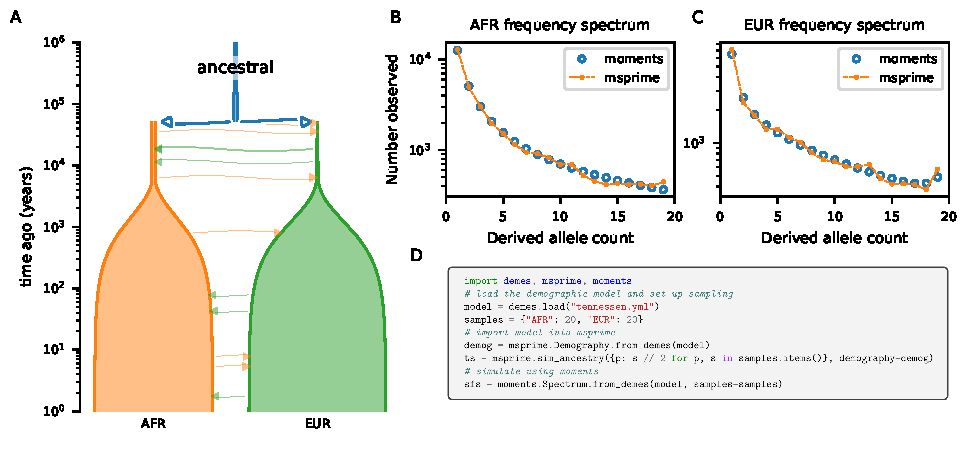
\includegraphics{fig/showcase}
    \caption{
        \textbf{Illustration and simulation using Demes.}
        (A)
        Using an inferred demographic model from \citet{tennessen2012evolution}
        specified as a YAML file in Demes format (Figure~\ref{fig:tennessen}), we
        used \demesdraw\ to visualize the demographic model (note the recent
            exponential growth resulting in present-day population sizes that
        greatly exceed those in the past).
        We then used \msprime\ to simulate genomic data for 20 genome copies
        sampled from the two contemporary populations, and we used \moments\
        to compute the expected joint site-frequency spectrum for the same
        sample sizes (Figure~\ref{fig:tennessen-simulation}).
        (B, C) We compared the single-population SFS in each population, showing
        agreement between the simulation methods.
        (D) Python code snippets of the interactions between \demes\ and the simulation
        software. An extended script to compute the SFS shown in (B) and (C) is
        given in Figure~\ref{fig:tennessen-simulation}.
    }
    \label{fig:showcase}
\end{figure}

Here, we highlight the interaction between Demes and other software, including
simulation and model illustration tools. Demes allows us to specify a
demographic model which can be used as the input for a growing
number of simulation packages (Table~\ref{tab:software}). We implemented the
human two-population demographic model from \citet{tennessen2012evolution}
inferred from European and African-American sequencing data. This model (shown
in Demes format in Figure~\ref{fig:tennessen}) is parameterized by an ancestral
population with an ancient growth, divergence into ``AFR'' and ``EUR'' that
each have multiple-epoch size histories, and multiple epochs of continuous
migration between the two branches (illustrated using \demesdraw\ in
Figure~\ref{fig:showcase}A). The large final sizes (\(\approx 500,000\)
individuals each) are one to three orders of magnitude larger than ancestral
population sizes, reflecting the recent explosive population size increase in
humans.

We used this model to simulate 20 haploid genome copies from EUR and AFR
at time zero (i.e., present day) to obtain the joint site-frequency spectrum
(SFS), a summary of observed allele frequencies widely used in evolutionary
inference
\citep{bustamante2001directional,gutenkunst2009inferring,tennessen2012evolution,
jouganous2017inferring,kamm2017efficient,kim2017inference}.
The Demes model (Figures~\ref{fig:showcase}A~and~\ref{fig:tennessen}) was
provided as the input demography to \msprime\ \citep{baumdicker2021-iu} to
simulate a large recombining region under the mutation rate assumed in
\citet{tennessen2012evolution}, and we computed the observed SFS using \tskit\
\citep{ralph2020efficiently}. Using the same Demes model as input to \moments\
\citep{jouganous2017inferring}, we computed the expectation of the joint SFS
and compared to the \msprime\ simulated data (Figure~\ref{fig:showcase}B,C).
Figure~\ref{fig:showcase}D shows the code required to run the
simulations in \msprime\ and \moments, and demonstrates that
precisely the same input model, without modification, was provided to both packages.
Such interoperability is a major gain for researchers, which we
hope will become the expected norm as more packages adopt the Demes
format.

\section*{Discussion}
Stable and healthy software ecosystems require standard interchange
formats, allowing for the development of high-quality and long-lasting
tools that produce and consume the standard.
Demographic models are a key part of population genetics research,
and to date the transfer of inferred models to downstream simulations
has been \textit{ad-hoc}, and conversions between the many different ways
of expressing such models is both labor intensive and error-prone.
The proposed Demes standard is an attempt to bridge this gap
between inference and simulation, and also to provide the foundations
for a sustainable ecosystem of tools built around this data model.
Table~\ref{tab:software} shows some initial infrastructure that we have
built as part of developing Demes, but many other useful tools
can be envisaged that produce, consume, or transform this format.

Reproducibility is a significant problem throughout the
sciences~\citep{baker20161}, and various measures have been
proposed to increase the likelihood of researchers being
able to replicate results in the
literature~\citep{munafo2017manifesto}. The most basic requirement
for reproducibility is that we must be able to state precisely what
the result in question \emph{is}. The lack of standardization in how
complex demographic models are communicated today, and the lack of
precision in the published model descriptions means that it is difficult
to replicate analyses, or reproduce those models for later simulation.
Thus, we hope that the Demes standard introduced here will be widely adopted
by simulation and inference methods and be used for reporting results in
publications, either as supplemental material or uploaded to a data repository.

\section*{Acknowledgments}
Graham Gower was supported by a Villum Fonden Young Investigator award to Fernando Racimo (project no. 00025300).
Ryan Gutenkunst was supported by the National Institute of General Medical Sciences of the National Institutes of Health (R01GM127348 to RNG).
Matthew Hartfield is supported by a NERC Independent Research Fellowship (NE/R015686/1).
Jerome Kelleher is supported by the Robertson Foundation.
Stephan Schiffels was supported by funding from the European Research Council (ERC) under the European Union’s Horizon 2020 research and innovation programme (grant agreement No 851511).

\bibliographystyle{genetics}
\bibliography{paper}

\renewcommand{\thefigure}{A\arabic{figure}}
\renewcommand{\thetable}{A\arabic{table}}
\renewcommand{\theequation}{A\arabic{equation}}
\renewcommand{\thesection}{A\arabic{section}}
\setcounter{figure}{0}
\setcounter{table}{0}
\setcounter{equation}{0}

\section*{Appendix}

The Demes specification is a formal data model for describing
the properties of populations over time,
along with some metadata and provenance information.
The data model is based on the ubiquitous JSON~\citep{bray2017javascript}
standard, and formally defined using
JSON Schema~\citep{wright2020json}.
Along with the schema, full technical details of the
of the model are provided in the
online specification document
(\url{https://popsim-consortium.github.io/demes-spec-docs/}).

\section{Population genetics model details}
\label{sec:appendix-pop-gen-model}

In Demes, demographic models consist of one or more interacting populations,
or ``demes'', understood to be a collection of individuals that can be
conveniently modeled using a defined set of rules and parameters
\citep{gilmour_demes_1939,gilmour_deme_1955}.
To avoid confusion with the name of the specification itself we will
use the term ``population'' in this discussion, with the understanding that the
terms are interchangeable.
A population is defined as some collection of individuals that exists for
some period of time, and has a well-defined size (i.e., number of individuals)
during that time period. Individuals can move between populations
either according to their ancestor-descendant relationships
or through processes involving migrations.
Few other properties of the populations are specified in the model:
we are concerned primarily with defining the populations, their sizes, and the
movement of individuals between those populations.

\subsection{Time units}

Population and event times are written as units in the past, so that time zero
corresponds to the final generation or ``now'', and event times in the past are
values greater than zero with larger values corresponding to times in the more
distant past. By having time values increase into the past, we avoid the need to
choose an arbitrary point in history as ``time zero''. A natural
specification for time units is in generations, although other time units are
permitted, such as years, accompanied by the generation time
so that downstream software may convert times into generations as required.

There must be at least one population with an infinite \texttt{start\_time}.
An infinite start time may be interpreted differently depending on the simulator.
In a coalescent setting, there is no upper bound for the coalescent time
of lineages in this population.
In a forwards-time setting, the interval of time between infinity and
the oldest non-infinite model time (i.e. the ``first event") is approximated
by the simulator's burn-in phase---detailed guidance
is provided in the online specification.

\subsection{Sizes and epochs}

Population sizes are given as numbers of individuals, and details
such as ploidy levels are considered external to the model.
We therefore focus on the number of individuals as opposed
to the number of genome copies.
Sizes and mating system details are specified for each population within
population-specific epochs.
Epochs are contiguous time intervals that define
the existence interval of the population. Each epoch specifies the population size
over that interval, which can be a constant value or a function defined by start
and end sizes that must remain positive.
Only exponential population size changes are currently supported,
but other functions may be added to the specification over time.


\subsection{Population dynamics}
\label{sec:appendix-population-dynamics}
Within a population, we assume that allele frequency dynamics can
be described by the Wright-Fisher model.
Briefly, generations are non-overlapping (all parents
reproduce and die simultaneously), and for allele $i$ currently at frequency $p_i$,
its frequency in the next generation (at birth) is expected to be $p_iw_i/\bar{w}$,
where $w_i$ and $\bar{w}$ are the marginal and
mean fitnesses, respectively, properly weighted according to ancestry proportions.
In this framework,
a forward-time simulation of finite populations is equivalent
to multinomial sampling of allele frequencies each
generation (\citet[][pp 29-31]{burger2000-ul}, \citet[][pp 179-181]{crowkimura1970}),
and a backwards-time (coalescent) simulation follows the approximations
described in \citet{tajima1983evolutionary,hudson1983testing}
and \citet[][chapter 3]{wakeley2008-hd}.
Further, this model assumes ``soft'' selection \citep{christiansen1975hard},
meaning that the dynamics of population sizes
changes are independent of the details of individual fitnesses.
As such, this model excludes scenarios such as ``hard selection,''
in which population sizes are dependent on a population's mean fitness, or
stochastic fluctuations in population size, such as interpreting
population sizes as carrying capacities.
Many forwards and backwards time simulators currently implement this model
\citep[e.g.,][]{hudson2002generating,gutenkunst2009inferring,excoffier2011fastsimcoal,kelleher2016efficient,jouganous2017inferring,haller2019slim,thornton2019-nu}.

\subsection{Selfing and cloning}

Each population has an assigned selfing rate and cloning rate, where each defines
the probability that offspring are generated from one generation to the next by either
self-fertilization or cloning of an individual.
More specifically, for a given epoch within a population denote the clonal rate by
$\sigma$ and the selfing rate by $S$.
$S$ and $\sigma$ can take any value between zero and one and
can sum to more than one.
Each generation a proportion of offspring
$\sigma$ are expected to be generated through clonal reproduction,
while $1-\sigma$ are expected to arise through sexual reproduction.
Within the sexually-reproduced offspring,
a proportion
$S$ are born via self-fertilization while the rest
have parents drawn at random from the previous generation.
Depending on the simulator, this random drawing of parent may occur
either with or without replacement. When drawing occurs with replacement, a small
amount of ``residual'' selfing is expected, so that the realized selfing probability
is $(1-\sigma)(S + (1-S)/N)$ instead of $(1-\sigma)S$ (so that even with $\sigma=0$
and $S=0$, selfing may still occur with probability $1/N$), although
this effect is negligible in large populations \citep{nordborg1997coalescent}.

By allowing the definition of selfing and cloning probabilities, we allow many
standard models to be defined.
However, by parameterizing selfing and cloning as we have, we assume that these
properties of populations can be specified independently from the genetics.
In other words, mutations that cause selfing probabilities to fluctuate within
an epoch are not considered.
More details of the mathematical properties of selfing and cloning rates
in a coalescent context can be found in
\citet{nordborg1997coalescent,hartfield2016facsexcoal}.

\subsection{Relationships between populations}

A population may have one
or more ancestors, which are other populations that exist at the population's
start time. If one ancestor is specified, the first generation is constructed
by randomly sampling parents from the ancestral population to contribute to
offspring in the newly generated population. If more than one ancestor is
specified, the proportions of ancestry from each contributing population must
be provided, and those proportions must sum to one. In this case, parents are
chosen randomly from each ancestral population with probability given by those
proportions.

Individuals in a population may have parents from a different
population through migrations. These can be defined as continuous migration
rates over time intervals for which populations coexist or through
instantaneous (or pulse) migration events at a given time. Continuous migration
rates are defined as the probability that parents in the ``destination''
population are chosen from the ``source'' population.
On the other hand, pulse
migration events specify the instantaneous replacement of a given fraction of
individuals in a destination population by individuals with parents from a
source population.


\section{Rationale for YAML}\label{sec:appendix-spec}

We have adopted the widely
used YAML format~\citep{ben2009yaml} as the recommended means of interchanging
Demes models (e.g., Figures~\ref{fig:IM}~and~\ref{fig:tennessen}). YAML is a data
serialization language with an emphasis on simplicity and which interoperates well
with JSON (indeed, YAML 1.2 is a superset of JSON). We chose YAML over JSON
because although JSON is an excellent format for data interchange, it is
ill-suited for human understanding and manipulation. We also considered other
declarative data exchange formats such as TOML,
but chose YAML because of its equivalence with JSON,
popularity, and good software support.
Since the Demes data model is defined in JSON Schema,
however, there is no formal dependency on YAML and implementations may choose
to use JSON directly if they wish (e.g., for greater efficiency).

\section{Rationale for static models}
\label{sec:appendix-static}

The Demes specification is designed to describe demographic
models defined by a fixed set of model parameters.
As described in the main text, it does not include
information about estimated confidence intervals or the joint distribution
of parameter values. In this section we describe the rationale
for this design decision.

The parameters of
demographic models are typically tightly coupled, and cases in which
distributions for different parameters can be simply described are rare.
In this situation, the simplest way to describe an estimated
distribution is to list a large number of samples from
the posterior. While writing out a large number of Demes models in
YAML format may seem inefficient, it can in fact be a compact
way to describe these distributions.
For example, consider a one-population model with piecewise-constant sizes over
20 epochs which has $\sim$~40 free parameters: the \texttt{start\_size} and
\texttt{end\_time} values for each epoch. If we sample 50,000 models
from the posterior distribution, the resulting multi-document YAML file is
45~MiB.
This format compresses down to 8.4~MiB when gzipped or 6.2~MiB
when compressed with LZMA2, which is on par with an equivalent binary
representation of the free parameters
($40\times50000\times4~\text{bytes} \approx 7.6~\text{MiB}$).

Similarly, one might be interested in running simulations in which
the demographic model parameters are drawn from a distribution, e.g.,
in ABC inference~\citep{beaumont2002approximate}.
Other inference procedures based on optimizing a loss function
\citep{gutenkunst2009inferring,kamm2017efficient,jouganous2017inferring,ragsdale2019models,excoffier2021fastsimcoal2}
%(\ggcomment{more refs? MCMC? neural networks?})
need users to specify parameter bounds,
and possibly non-linear or conditional constraints between parameters.
Indeed, the choice of how to parameterize a model could be important for
some inference methods (e.g. absolute times versus relative times between events).

Implementing the many distributions of interest and supporting a general
way to describe a model's free parameters would greatly increase the
complexity of parsers, with relatively limited benefit to most users.
It is unlikely that Demes could be made sufficiently
flexible without implementing many features of
general-purpose programming languages, such as variables, arithmetic,
and flow control.
Such use cases are therefore better served by writing model-generating
functions in an existing programming language, for example
using the Demes Python API (e.g., as implemented in \moments\
\citep{jouganous2017inferring,ragsdale2019models}).
%To modify an existing static Demes model, perhaps to infer new parameters,
%this would unfortunately require reimplementing the model.
As an intriguing possibility for developments in this direction,
there exist many templating solutions for YAML and JSON that are
specifically designed for extending static data in arbitrarily complex ways
(e.g., \texttt{YTT}, \texttt{Jsonnet}, \texttt{CUE}, and \texttt{Dhall}).
%\citep{ytt,jsonnet,cue,dhall}.
%(\ggcomment{refs: YTT, Jsonnet, CUE, Dhall}).


\section{Extended data and figures}
\label{sec:appendix-figures}

\begin{figure}[h!]
    \begin{tcolorbox}
        \inputminted[fontsize=\scriptsize,numbersep=5pt]{yaml}{models/IM-resolved.yaml}
    \end{tcolorbox}
    \caption{
        \label{fig:IM-MDM}
        Isolation-with-migration example model from Figure~\ref{fig:IM}
        in Machine Data Model (MDM) form.
        The MDM form of the model is complete and explicit, but contains
        much redundant information that is omitted in the Human Data Model
        (HDM) form.
    }
\end{figure}

\begin{figure}[h!]
    \begin{tcolorbox}
        \inputminted[fontsize=\scriptsize,numbersep=5pt]{yaml}{models/tennessen.yaml}
    \end{tcolorbox}
    \caption{
        \textbf{The \citet{tennessen2012evolution} two-population
        demographic model in Demes format.}
        This model includes a single ancestral population that expands in
        size in the past, followed by divergence between AFR- and EUR-labeled
        populations. The two-population phase of the model includes multiple
        epochs of varying size, and rapid exponential growth over the past
        five thousand years in each population.
    }
    \label{fig:tennessen}
\end{figure}

\begin{figure}[h!]
    \begin{tcolorbox}
        % NOTE: line highlights may need adjusting after changing this code
        \inputminted[fontsize=\scriptsize,numbersep=5pt,highlightlines={9,19,52}]{python}{models/tennessen-simulation.py}
    \end{tcolorbox}
    \caption{
        \textbf{Simulation of SFS for the Tennessen model.}
        We first load the demographic model using \demes\ (as \texttt{graph}),
        which can then be used by \msprime\ to create the demographic model used in
        \texttt{msprime.sim\_ancestry()}. The same loaded graph can also be
        passed to \moments\ to compute the expected joint SFS.
        To compare the SFS in Figure~\ref{fig:showcase}, we marginalize the
        joint SFS to obtain the single-population SFS for both AFR and EUR populations.
        Lines interfacing \demes\ and other software are highlighted.
    }
    \label{fig:tennessen-simulation}
\end{figure}


\end{document}
